\chapter{LINUX}
\label{apa:linux}
\vspace{-2cm}

Neste capítulo será abordado o surgimento e a evolução do sistema operacional Linux. \cite{garver_sept70}.

\section*{\hspace{1.3cm}APÊNDICE A.1 - HISTÓRICO DO LINUX}
\label{secapa:linux}
Atualmente, ... 

Segundo \citeonline{machado}, o sistema operacional (SO), possui inúmeras funções, as quais podem ser resumidas em duas:
\begin{itemize}
\item \textbf{Facilidade de acesso aos recursos:} consiste em ser totalmente transparente ao usuário a maneira como funciona um computador \index{computador} paralelo \index{computador!paralelo} , ou seja, para um usuário não importa como um arquivo que está em um disquete será lido, mas sim que o mesmo será lido, resumindo, um usuário \index{usuário} não precisa saber como será realizado essa ação e suas inúmeras etapas;
\end{itemize}

%\begin{figure}[htbp]
%\begin{figure}[H]
%\tiny \caption[Ilustração é um exemplo de figura]{\small Ilustração.} % o que está dentro dos colchetes é o que vai aparecer na lista de figuras. Tenha essa possibilidade a mais, veja que a figura do capítulo 2 está diferente.
%\vspace{-0.3 cm}
%\begin{center}
%\begin{psfrags}
%\epsfxsize=4cm
%\centerline{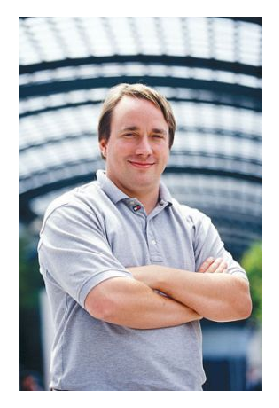
\includegraphics[width=4.0 cm]{./apa/linus_torvalds.eps}}
%\end{psfrags}
%{\small Fonte: Adaptado de \citeonline{machado}}
%\end{center}
%\label{torvalds}
%\end{figure}
%
